\documentclass[final]{siamart1116}

%% ------------------------------------------------------------------
%% Code used in examples, needed to reproduce 
%% ------------------------------------------------------------------
%% Used for \set, used in an example below
\usepackage{braket,amsfonts}
\usepackage{graphicx}
\usepackage{wrapfig}
%% Used in table example below
\usepackage{array}

%% Used in table and figure examples below
\usepackage[caption=false]{subfig}
%% Used for papers with subtables created with the subfig package
\captionsetup[subtable]{position=bottom}
\captionsetup[table]{position=bottom}

%% Used for PgfPlots example, shown in the "Figures" section below.
\usepackage{pgfplots}

%% Used for creating new theorems, remarks
\newsiamthm{claim}{Claim}
\newsiamremark{rem}{Remark}
\newsiamremark{expl}{Example}
\newsiamremark{hypothesis}{Hypothesis}
\crefname{hypothesis}{Hypothesis}{Hypotheses}

%% Algorithm style, could alternatively use algpseudocode
\usepackage{algorithmic}

%% For figures
\usepackage{graphicx,epstopdf}


%% For referencing line numbers
\Crefname{ALC@unique}{Line}{Lines}

%% For creating math operators
\usepackage{amsopn}
\DeclareMathOperator{\Range}{Range}

%strongly recommended
\numberwithin{theorem}{section}

%% ------------------------------------------------------------------
%% Macros for in-document examples. These are not meant to reused for
%% SIAM journal papers.
%% ------------------------------------------------------------------
\usepackage{xspace}
\usepackage{bold-extra}
\usepackage[most]{tcolorbox}
\newcommand{\BibTeX}{{\scshape Bib}\TeX\xspace}
\newcounter{example}
\colorlet{texcscolor}{blue!50!black}
\colorlet{texemcolor}{red!70!black}
\colorlet{texpreamble}{red!70!black}
\colorlet{codebackground}{black!25!white!25}

\newcommand\bs{\symbol{'134}} % print backslash in typewriter OT1/T1
\newcommand{\preamble}[2][\small]{\textcolor{texpreamble}{#1\texttt{#2 \emph{\% <- Preamble}}}}

\lstdefinestyle{siamlatex}{%
  style=tcblatex,
  texcsstyle=*\color{texcscolor},
  texcsstyle=[2]\color{texemcolor},
  keywordstyle=[2]\color{texemcolor},
  moretexcs={cref,Cref,maketitle,mathcal,text,headers,email,url},
}

\tcbset{%
  colframe=black!75!white!75,
  coltitle=white,
  colback=codebackground, % bottom/left side
  colbacklower=white, % top/right side
  fonttitle=\bfseries,
  arc=0pt,outer arc=0pt,
  top=1pt,bottom=1pt,left=1mm,right=1mm,middle=1mm,boxsep=1mm,
  leftrule=0.3mm,rightrule=0.3mm,toprule=0.3mm,bottomrule=0.3mm,
  listing options={style=siamlatex}
}

\newtcblisting[use counter=example]{example}[2][]{%
  title={Example~\thetcbcounter: #2},#1}

\newtcbinputlisting[use counter=example]{\examplefile}[3][]{%
  title={Example~\thetcbcounter: #2},listing file={#3},#1}

\DeclareTotalTCBox{\code}{ v O{} }
{ %fontupper=\ttfamily\color{texemcolor},
  fontupper=\ttfamily\color{black},
  nobeforeafter,
  tcbox raise base,
  colback=codebackground,colframe=white,
  top=0pt,bottom=0pt,left=0mm,right=0mm,
  leftrule=0pt,rightrule=0pt,toprule=0mm,bottomrule=0mm,
  boxsep=0.5mm,
  #2}{#1}

% Stretch the pages
\patchcmd\newpage{\vfil}{}{}{}
\flushbottom

%% ------------------------------------------------------------------
%% End of macros for in-document examples. 
%% ------------------------------------------------------------------

%% ------------------------------------------------------------------
%% HEADING INFORMATION
%% ------------------------------------------------------------------
\begin{tcbverbatimwrite}{tmp_\jobname_header.tex}
\title{Guide to Using SIAM's \LaTeX\ Style%
  \thanks{Submitted to the editors DATE.
\funding{Funding information goes here.}}}

\author{Dianne Doe%
  \thanks{Imagination Corp., Chicago, IL (\email{ddoe@imag.com}).}%
  \and
  Paul T. Frank%
  \thanks{Department of Applied Math, Fictional University, Boise, ID
    (\email{ptfrank@fictional.edu}, \email{jesmith@fictional.edu}).}
  \and
  Jane E. Smith%
  \footnotemark[3]
}

% Custom SIAM macro to insert headers
\headers{Guide to Using  SIAM'S \LaTeX\ Style}
{Dianne Doe, Paul T. Frank, and Jane E. Smith}
\end{tcbverbatimwrite}
\input{tmp_\jobname_header.tex}

% Optional: Set up PDF title and authors
\ifpdf
\hypersetup{ pdftitle={Guide to Using  SIAM'S \LaTeX\ Style} }
\fi

%% ------------------------------------------------------------------
%% END HEADING INFORMATION
%% ------------------------------------------------------------------

%% ------------------------------------------------------------------
%% MAIN Document
%% ------------------------------------------------------------------
\begin{document}

%\maketitle


%% ------------------------------------------------------------------
%% ABSTRACT
%% ------------------------------------------------------------------
\begin{tcbverbatimwrite}{tmp_\jobname_abstract.tex}
\begin{abstract}
	In traditional multigrid, the number of unknowns on refined domains can create a memory bottleneck. The memory requirements can also reduce the efficiency of the algorithm due to the communication required between cores. I analyze Segmental Refinement Multigrid (SRMG) a modification to multigrid methods that reduces communication and has logarithmic scaling memory complexity. While previous work has been done on this method, and there have been earlier implementations, they all failed to converge on an arbitrary number of levels. My work provides a theoretical analysis and practical implementation demonstrating the root cause of SRMG's previous failures was due to the underlying low-communication mechanisms of the algorithm. My concluding analysis demonstrates future potential for SRMG, although it imposes requirements that could not be met by the implementation accompanying this work. 
\end{abstract}

\begin{keywords}
 Multigrid, Segmental Refinement
\end{keywords}

\begin{AMS}
 \textbf{Lookup comp math}
\end{AMS}
\end{tcbverbatimwrite}
\input{tmp_\jobname_abstract.tex}
%% ------------------------------------------------------------------
%% END HEADER
%% ------------------------------------------------------------------

\section{Introduction}\label{sec:intro}
%   1) Introduction
%   2) Background (put citations of previous work here), not significance of
% problem
%   3) Methodology (proofs go here)
%   4) Results (graphs and pictures go here)
%   5) Conclusions (hand waving goes here)
  
  Here we study a low-memory modification of multigrid methods, which are a class of methods for
solving partial differential equations. This modified multigrid method, Segmental Refinement (SRMG) \cite{brandt1994multigrid}, reduces concurrent memory requirements by creating an overlapping domain decomposition and independently solving the partial differential equation on each subset of the domain. Error imposed by this method exists only in the overlapping region, or buffer region, and requires only modest additional computation in the redundant overlap between domains. This overlapping decomposition is the reason SRMG has logarithmic scaling memory requirements rather than the linear scaling memory requirements of traditional multigrid.
    
\begin{wrapfigure}{r}{0.4\textwidth}
  \begin{center}
    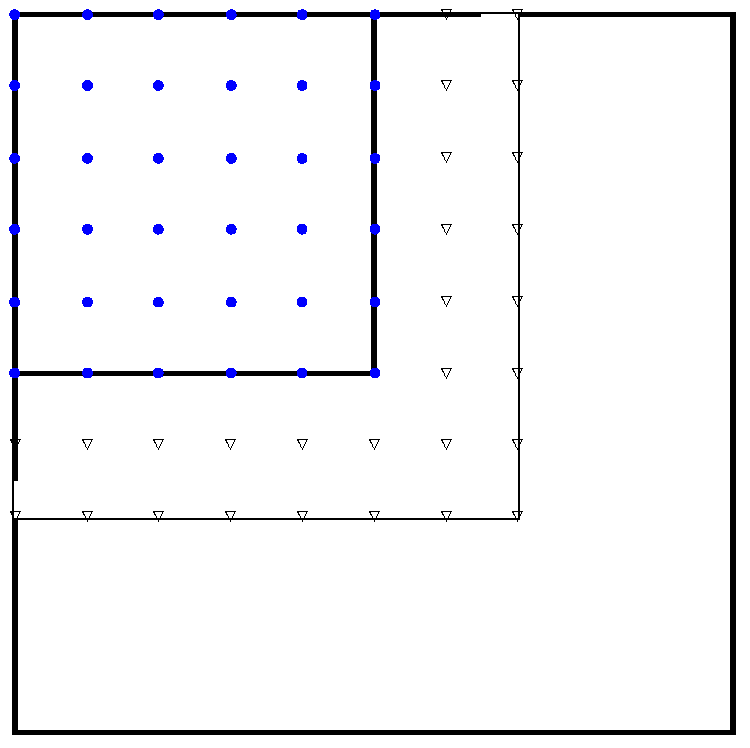
\includegraphics[scale=0.4]{sketchsr.pdf}
  \end{center}
  \caption*{\textbf{JRT:Get better picture} \footnotesize{Significant error is constrainted to triangular black points}}
\end{wrapfigure}


	Previous analysis and implementation demonstrated that SRMG could work for some fixed number of levels \cite{paper1}, but my work attempts to demonstrate that convergence holds for any number of levels of SRMG, so long as each level eliminates low-frequency error and further levels maintain this high-frequency accuracy. 
    
	There are two unanswered questions regarding SRMG. One is whether we have convergence guarantees in spite of communication no longer occuring between patches.  I show error induced by no longer communicating with the entire domain is localized and does not extend past the buffer regions of the domain decomposition. 
    
	The second question is whether SRMG converges on an arbitrary number of refinement levels. I demonstrate a set of requirements which, when satisfied, guarantee convergence on an arbitrary number of levels. I accompanied my analysis by implementing the method with a spectral solver, to investigate the feasibility of these requirements. 
    %but I demonstrate that if one is careful to account for modest param
    

\section{Background}\label{sec:backg}
By 1982, Multigrid was an accepted numerical algorithm for solving elliptic equations \cite{earlymulti}. The speed at which multigrid solves large problems is the primary reason for its use. One of the problems with multigrid, as well as many other numerical algorithms, is that memory requirements scales linearly. 
    
    For traditional multigrid methods, memory requirements scale linearly with the number of grid points on the highest-resolution domain. With the advent of multi-core machines, large problems can be solved by distributing memory loads across several cores. Parallel multigrid is one implementation of traditional multigrid that can distribute massive problems across several cores by partitioning the full domain into smaller, interdependent subdomains. However, parallel multigrid requires communication \cite{brandtdiskin} because the entire domain must be solved and the solution on each subdomain is dependent on the solution on neighboring subdomains.
    
    Even in some communication-efficient implementations of parallel multigrid, the high-resolution domain is partitioned into non-overlapping subdomains that must communicate. The  communication complexity of these algorithms scales linearly with the number of subdomains \cite{parallelcomm}. For especially difficult problems, the number of subdomains must be very large in order to fit each subdomain onto one core. Thus, the slowdown due to communication needs of parallel multigrid is especially noticeable. 
    
    An improvement upon parallel multigrid would be a method of solving partial differential equations that does not require communication between cores and requires less memory, all without sacrificing too much of the speed offered by traditional multigrid. 
    
    Segmental Refinement is an algorithm that finds a solution in only O($\log{N}$) memory, where N is the number of grid points on the full, highest resolution domain. Furthermore, the overlapping or buffer region of the decomposition into subdomains allows each subdomain to be solved indepedently, without communication with its neighbors. Thus, there is no communication required between the subdomains.
    	
	One may notice that since there are redundant grid points in the overlap of the SRMG subdomains, these redundant grid points increase the number of computations needed. However, my analysis shows that the size of this overlap is small relative to size of the problem, so the additional computations needed are a modest trade-off compared to the low-memory advantages. These additional computations are especially modest when one considers that they entirely eliminate the previously-discussed communication requirements of parallel multigrid, which scale with the number of subdomains distributed across the separate cores of a machine. In some instances, especially on machines with cores that are not efficient at horizontal communication, the overall computational time may be reduced \cite{id716}.
     
    Models of this SRMG algorithm were presented as early as 1994 \cite{brandtdiskin}. However, even now there is no software package written to perform SRMG for a user-provided differential equation, and there is still debate over what conditions must be met for the algorithm to have convergence. One question that had been left unanswered by previous research is whether Segmental Refinement can be performed an arbitrary number of times with arbitrarily small error. \cite{paper1}. 

	There has also been, without a software implementation, proof of convergence via segmental refinement with a fixed number of levels. However this proof is unaccompanied by numerical implementation on any specific differential equations and lacks strong evidence that unlimited levels of SRMG are possible \cite{brandtdiskin}. The theory  presented showed that error induced by one level of SRMG decays within the buffer region of each subdomain, but did not demonstrate that a buffer region of fixed size can still allow further levels of SRMG  without eventually inducing errors on the highest-resolution domains. However, this was an early work and still served to demonstrate that this algorithm had a potential use in reducing communication complexity during the last few stages of refinement when performing multigrid. In and of itself, this provided a significant, powerful use. Yet, it left unanswered the full potential of SRMG.
    
    
    
    Marcus Mohr provided further analysis in 2000, particularly focusing on how it can be used to reduce communication complexity when used on a multi-core machine and in some cases even reduce overall computation time. This continued to demonstrate the considerable advantages of such an algorithm. However, an implementation was still not given, and the model still did not account for arbitrary refinements. \cite{id716}. 
    
    Finally in 2015, an actual implementation was investigated \cite{paper1}. Analysis was done once again in depth, and with an accompanying numerical implementation, provided very strong support that SRMG had potential as a low-memory but reliable partial differential equation solver. Furthermore, code performing the algorithm was made publicly available, including all the data on which the researches experimented. While the code was experimental and not designed for use on new, user-defined problems, the research done by these authors demonstrated even further the potential of SRMG.
    
    In their work, the researchers discovered that convergence depended on an additional parameter not previously considered \cite{paper1}. In their  implementation of SRMG, the authors found that increasing the resolution of the coarsest level on which SRMG is used proportionally decreased the error induced by SRMG and also the buffer region required to achieve convergence on the interior of each subdomain. Previous analysis made no connection between the resolution on the coarsest grid and the error induced by subsequent levels of SRMG.
    
    While convergence was shown in the 2015 implementation for SRMG up to a few levels, there was no evidence suggesting segmental refinement could or could not be performed indefinitely. Errors grew beyond acceptable levels unless the buffer size grew as compensation. Increasing the buffer size also increases the memory requirements and computational complexity of SRMG. Therefore, a requirement that buffer size grow with the number of SRMG levels would undermine the advantages offered by using this algorithm in place of parallel multigrid. Even worse, it was unclear whether a large number of SRMG levels would necessitate a buffer region extending beyond the boundaries of the original problem. It was also not clear what was causing convergence failures under different circumstances, and whether they could be ameliorated while preserving the low-memory, high-speed properties of SRMG. 
    
    My work builds upon this body of previous work by approaching the analysis of the algorithm from a new perspective, showing that convergence depends on the number of unknowns solved for on the coarsest level as well as the on solver used. In order for SRMG to be effective, one must eliminate all low-frequency errors on coarser patches. That means, at a minimum, one must use a solver that does not induce interpolation error.  Additionally, one must solve on a sufficiently high-resolution grid before commencing SRMG levels. Failure to meet both of these conditions can cause errors to propagate into the decomposed domain. 
    
    Our analysis shows that error induced by SRMG decays exponentially with respect to the frequency of error on the boundary. Thus, a sufficiently high-resolution domain must be solved before commencing SRMG so that low-frequency errors are eliminated. Furthermore, the solver used must not reintroduce low frequency errors when moving from low to high resolution grids. When combined, these two properties force errors to decay to the level of second order discretization error in the buffer region, so that our solution converges within the area of interest of each subdomain.  
    
   
    
%     We demonstrate that when a solver is used that does not induce interpolation error (e.g. Fourier Transform) and if a sufficiently large number of unknowns are solved for on the entire domain, one can commence with segmental refinement without introducing error above the order of discretization error. 
    
    
    The results from my analysis and implementation support the work done in 2015 by demonstrating why the buffer needed to grow with SRMG in order to guarantee convergence. Because the coarsest grid does not solve for a sufficient number of unknowns when levels begin using SRMG, low-frequency errors are induced on each buffer.  Furthermore, the solver they use induces interpolation error, thus low frequency errors are introduced at each new level of SRMG. 
    
    Since low-frequency errors are coming from the coarsest SRMG level and each interpolation from high to low resolution domains, the method induces low frequency errors at the boundary of each buffer region. These low-frequency errors propagate further into each subdomain than high-frequency errors. Thus, the buffer size has to grow much larger to compensate for the long-distance propagation of these errors. My analysis shows that these low-frequency errors are a probable cause for convergence failures in the aforementioned implementation \cite{paper1}. Furthermore, my analysis improves the robustness of the algorithm by deriving explicit error bounds. 
    
    % than would be necessary for my proposed modifications.
    
    With some information about the magnitude of frequencies of the true solution to a problem (more precisely, bounds on the high-frequency Fourier coefficients), one can find exactly how many unknowns must be solved for on the entire domain before one can switch from solving coarse grids via traditional multigrid to taking advantage of the low-memory SRMG algorithm on all subsequent high resolution domains. Through numerical experiments, I find that the number of unknowns which must be solved is tractable and will still require much less memory than traditional multigrid.
    
    Note that my analysis demonstrates that it is critical for the method used not to induce any interpolation error. A method such as finite differences  would induce interpolation error, which would allow low-frequency errors to enter highly refined grids. 
    %({\bf MGK:} Note that these low-frequency errors are normally reduced by iteration, which we do not use here, but [Adams 2016] does. We should think a little more about this comment in relation to the iterative vs non-iterative formulation. {\bf Response: Something like} "Note that my spectral solver also uses a direct method to solve for the approximate solution, whereas the typical approach uses an iterative method to reduce low-frequency errors and then performs several cycles. " ) 
    %the prior code did not solve with a spectral method, 
    
	Finally, I demonstrate that SRMG scales logarithmically with the number of unknowns. I show that my aforementioned proposals for adjustments to prior implementations do not increase the scaling of SRMG's memory requirements, even with an arbitrary number of levels. 
    
    
    To  demonstrate the true value of SRMG, I implement an algorithm with a spectral solver in order to observe whether convergence can hold for a high number of levels. Note that this solver is not implemented in the true spirit of multigrid. Each solve is performed directly, rather than through an iterative method. However, the nature of this implementation was exploratory, intended to isolate possible sources of previous multi-level convergence failures. Furthermore, I take advantage of my preliminary analysis to determine requisite buffer sizes and coarse resolutions required to achieve multi-level convergence. 
    
    Upon review of the numerical results, it was clear that multi-level convergence was not occuring consistently. However, this eliminated the theory that interpolation error was the reason for SRMG requiring a buffer that grows with the number of levels desired. 
    
    There were many possible reasons for this multi-level convergence failure, so I performed a second, more abstract analysis in light of these results. Error induced by the first artificial boundary condition imposed on the first level of SRMG cannot not be eliminated by refinement, only by increasing coarsest resolution or buffer size. However, this is not the death of multi-level SRMG. My analysis also demonstrates how to set up SRMG to achieve a pre-determined level of accuracy on the highest-resolution domains. In fact, it is possible that guaranteeing error decays to machine-epsilon yields convergence on an arbitrary number of levels. While this is a stronger requirement than originally considered, it is not wholly infeasible. And it can be shown that, so long as subsequent levels continue to generate high-frequency accuracy on their interior, a fixed buffer size can allow convergence on an arbitrary number of levels of SRMG. Unfortunately, the implementation  provided in, and computational resources available for, this work were not suitable for this newfound set of requirements. 
    
    
    The value of the analysis done in this thesis is two-fold: finding the cause of previous limitations on implementations of SRMG and also investigating the necessary modifications needed to remove these limitations. A next step would be to implement a more sophisticated method for Segmental Refinement, one capable of removing all sources of low-frequency error, and one that genereates overlapping domain decompositions with a buffer size large enough to accomodate the added requirements for Segmental Refinement to achieve multi-level convergence.  
    
    It remains to be shown that an implementation eliminating all sources of low-frequency error would still yield a reasonably fast application for solving Poisson's equation. However, software designed to meet these convergence requirements, if made publicly available, will allow one to solve Poisson's equation in O($\log{N}$) memory.  This allows once-unsolvable problems to be solved, both for individual researchers with a dearth of resources and organizations with a plethora of computational power. Memory will no longer be a bottleneck for computations done via multigrid, and there will only be a small increase in the number of computations that must be done, but with significantly decreased communication complexity.
   

\section{Methodology}\label{sec:method}
\subsection{Model Problem}
%    ({\bf MGK:} The notation much be unified in the whole document. Will you use $u$ or $\Phi$ as the unknown? What notation for the Laplacian?)
Consider Poisson's equation on the domain $[0, 1]$ x $[0, 1]$

\begin{gather}
  \bigtriangleup  u(x,y) = f \label{eq:Poisson} \\
  \begin{split}
    u(0,y) &= u_{west}(y) \quad u(1,y) = u_{east}(y) \label{boundary} \\
    u(x,0) &= u_{south}(x) \quad u(x,1) = u_{north}(x) \nonumber
  \end{split}
\end{gather}


% \begin{align}\label{eq:Poisson}
%  \bigtriangleup u = f
% \end{align}
We can attempt to solve this problem numerically using multigrid. 

    %Suppose we used a second-order discretization and an exact (e.g. spectral) solver.     
Discretizing (\ref{eq:Poisson}) by a spectral method and solving using a multigrid method yields an approximate solution with a Fourier representation that is accurate up to the first $k$ modes. To increase the value of this $k$, one can solve on a more refined grid using the approximation generated on a coarse grid as an initial guess for the solution on the refined discretization. 

We consider a modification of multigrid: segmental refinement, which solves for the refined domain by locally solving on patches of an overlapping decomposition of the domain. 

%({\bf MGK:} When you refer to an equation parameter in the text, always use math mode).
A brief outline of the SRMG method is:

\begin{enumerate}
\item Solve coarse grid 
\item Quarter grid into four patches
\item Extend boundary of patch to include buffer region. 
\item Refine each patch
\item Solve on patch, then repeat steps 2-4 on this new patch. 
\end{enumerate}

\subsection{Justification of Convergence}\label{sec:firstanalysis}

The SRMG algorithm crucialy relies on the accuracy of the solution far from the boundary. If error decays sufficiently
rapidly away from a boundary, then an inexact boundary condition combined with a buffer region can be used to obtain an
accurate solution inside the domain. 

To this end, we will look at the decay of the solution to the Laplace equation on a square domain with boundary values driven by high-frequency errors. Assume that step 1 of SRMG is completed, meaning a coarse solution  $u^{(0)}(x, y)$ is generated as an approximation to the true solution. This coarse solution $u^{(0)}$ is used to impose boundary conditions on the patches generated by steps 2 and 3. 

Consider in specific the patch solution $u^{(1)}$ generated on the lower left patch $[0, L]$ x $[0, L]$, which interfaces with the true boundary on the West and South but is given by artificially boundary conditions  on the other two sides. 

\begin{gather}
  \bigtriangleup  u^{(1)}(x,y) = f  \\
  \begin{split}
    u^{(1)}(0,y) &= u_{west}(y) \quad u^{(1)}(L,y) = u^{(0)}(L, y) \\
    u^{(1)}(x,0) &= u_{south}(x) \quad u^{(1)}(x,L) = u^{(0)}(x, L) \nonumber
  \end{split}
\end{gather}

Let the error between the true solution and the coarse solution be given by $E^{(0)}(x, y) = u^{(0)}(x, y) - u(x, y)$

We can therefore analyze the error on this lower left patch, $E^{(1)}(x, y) = u^{(1)}(x, y) - u(x, y)$, resulting from this first SRMG decomposition  by expressing it as a solution to the following PDE: 

\begin{gather}
  \bigtriangleup  {E}^{(1)}(x,y) = \bigtriangleup u^{(1)} - \bigtriangleup u = f - f = 0 \\
  \begin{split}
    {E}^{(1)}(0,y) &= u_{west}(y) - u_{west}(y) = 0 \quad {E}^{(1)}(L,y) = u^{(0)}(L, y) - u(L, y) = E^{(0)}(L, y) \\
    {E}^{(1)} (x,0) &= u_{south}(x) - u_{south}(x) = 0 \quad E^{(1)}(x,L) = u^{(0)}(x, L) - u(x, L)  = E^{(0)}(x, L) \nonumber 
  \end{split}
\end{gather}



On $[0,L]\times[0,L]$. We can obtain a generic boundary condition by superposition of solutions satisfying one boundary conditions and three zero boundary value conditions. 

Therefore, we further simplify our analysis by individually evaluating the error imposed by one boundary. 

\begin{gather}
  \bigtriangleup  E(x,y) = 0 \label{laplaceexstate} \\
  \begin{split}
    E(0,y) &= 0 \quad u(L,y) = 0 \\
    u(x,0) &= 0 \quad u(x,L) = E^{(0)}(x, L) \label{laplaceexboundary} \nonumber 
  \end{split}
\end{gather}

This partial differential equation has series
solution \cite{Jackson1962}
\begin{align}
  E(x,y) &= \sum_{n=1}^{\infty} E_n(x,y) \label{errorinfreq} \\
            &= \sum_{n=1}^{\infty} B_n \sin\left(\frac{n\pi x}{L}\right) \sinh\left(\frac{n\pi y}{L}\right), \nonumber 
\end{align}
where the coefficients $B_n$ can be determined in terms of the inhomogeneous boundary condition, using the orthogonality of trigonometric functions. 

\begin{align*}
  B_n &= \frac{2}{L \sinh(n\pi)} \int^L_0 E^{(0)}(x, L) \sin\left(\frac{n\pi x}{L}\right) \,dx
\end{align*}

As one moves from the top boundary, the solution to this problem decays exponentially, which will motivate the size we require for our buffer used in SRMG.

%Suppose we bound the Fourier coefficients, which are encoded directly in $B_n$, of the boundary perturbation.  Or we state equivalently that we bound the energy in the perturbation, $C = \max_n |B_n|$. 


%\jeremy{Prove: that the max Fourier coefficient of $\Phi$ can never exceed that of $g$ since the Laplacian is smoothing.} 
% MGK NOT NOT UNDERSTAND: May also need to use parsevals due to aliasing
Thus we have the bound
\begin{align*}
\left|E_n(x, y)\right| &\leq \frac{2 B_n}{L \sinh(n\pi)} \sinh\left(\frac{n \pi y}{L}\right) \\
&\leq \frac{4 B_n}{L \cdot exp(n\pi)} exp({\frac{n \pi y}{L}}) \\
&\leq \frac{4 B_n}{L} exp({\frac{n \pi (y-L)}{L}}) 
\end{align*}
Letting $d = L-y$ be the distance from the boundary, we have
\begin{align}
  \left|E_n(x, y)\right| \leq \frac{4C}{L} exp({\frac{-n \pi d}{L}}), \label{errorbound}
\end{align}
and we see that the exponential decay away from the boundary is also exponential in the wavenumber of the perturbation.


%For our solution procedure, we assume that we obtain the exact solution on an initial coarse grid of size $n_0$. Further assume that each quarter of the domain encodes components corresponding to $n_0$ frequencies exactly.  
For our solution procedure, we assume that we obtain the solution on an initial coarse grid to remove any low-frequency errors. Thus along any artificial boundary of some form analogous to $y \in [0, L]$ and $x = L$ we have accuracy in the first $N_0$ Fourier components. That is the error corresponding to each wavefrequency, (\ref{errorinfreq}) is 0 for $n \leq N_0$.

Further assume that each quarter of the domain contains $N_0 \times N_0$ unknowns. 

We will number each grid starting with $l = 0$ for this coarsest grid. 

If we use a second order method for solving each finite-resolution patch, then the discretization error \footnote{To clarify any ambiguity, here our second order discretization error is defined as second order with respect to the distance between points or number of unknowns per unit area on a boundary, not cell size, which would actually be$(\frac{1}{k})^4$ . This is a trivial difference because the additional needed buffer size would at most double, or we could achieve this by doubling the coarse-solve accuracy $n_0$} at each level is $C_D \left(\frac{1}{2^l n_0}\right)^2$ for some constant $C_D$. If we double the resolution of our initial grid in each direction, but divide it into four patches, then at level $l = 1$ we have $L = \frac{1}{2}$ \footnote{Technically, SRMG must create a buffer zone, so $L = \frac{1}{2} + \epsilon$. We disregard this detail in the analysis provided here. }.



Let $C = \max{(|B_{n \leq 2N_0-1}|, \sum_{n=2N_0}^\infty |B_n|) } $

\begin{align}
  \left|E(x, y)\right| &\leq \sum^{\infty}_{n=N_0+1} |\frac{4 B_n}{L} exp(\frac{-n \pi d}{L})|  \nonumber \\  
& = \sum_{n=N_0+1}^{2N_0-1} |\frac{4B_n}{L} exp(\frac{-n \pi d}{L})| + \sum_{n=2N_0}^{\infty} |\frac{4B_n}{L} exp(\frac{-n \pi d}{L}) |  \nonumber \\
&\leq  \frac{4 C (N_0-1)}{L} exp(\frac{-N_0 \pi d}{L}) + \frac{4C}{L} exp(\frac{-N_0 \pi d}{L} ) \nonumber \\  
&= \frac{4C N_0}{L} exp(\frac{-N_0 \pi d}{L}) \nonumber \label{bound}  \\
\end{align}


%Since we assume that frequencies $1 \leq n \leq n_0$ are exact after interpolation, the approximation has no low-frequency errors. 

%Furthermore, we note that general multigrid eliminates low-frequency errors with coarse discretizations. So if the error imposed by SRMG is on the order of that imposed by multigrid, then each patch still eliminates low-frequency errors. Therefore, on each generated subpatch, we have only high-frequency error and can make an inductive argument as follows:


% Errors in the frequency range $n_0 \le n \leq 2n_0$ and can be bounded by the constant $C$. This bound must hold for at most the four edges of the patch, since later levels may generate interior patches that impose four artificial boundaries. 

Since later levels of SRMG may generate subpatches with up to four artificial boundaries, we require that the total error imposed by up to four erroneous boundaries be less than the discretization error at this level,

\begin{align}
  4 \frac{4C N_0}{L} exp(\frac{-N_0 \pi d_1}{L}) &< C_D \left(\frac{L}{N_0}\right)^2 \nonumber \\
 \implies  exp(\frac{-N_0 \pi d_1}{L}) &< \frac{C_D}{C} \frac{L^3}{16 N^3_0} \nonumber \\
  \implies d_1 &> -\frac{L}{N_0 \pi} \ln\left(\frac{C_D}{C} \frac{L^3}{16 N^3_0}\right) \nonumber \\
 \implies  d_1 &> \frac{\ln(C) - \ln(C_D) + (4+3) \ln(2) + 3 \ln(N_0)}{2^1 N_0 \pi}. 
\end{align}

This way, we can guarantee second-order discretization error on each patch. This is the same guarantee given by a second-order finite difference method, and multigrid with a finite difference discretization still eliminates low-frequency errors using the coarser grids. 

We continue to assume that refining each patch before quartering assures that each subpatch is generated with higher-frequency accuracy. We interpret this as an initial approximation on on all four subpatches that is exact up to the first $N_0$ components of the true Fourier representation of the given subpatch's boundary. That is (\ref{errorinfreq}) is still 0 for $n \leq N_0$, but L has shrunken, meaning the expression for the boundary-imposed error decays faster. 

On level $l$, let $d_l$ refer to the distance requirement at $l$ levels from the coarsest grid in order to have the error imposed by artificial boundaries decay to discretization error with respect to the given refinement. We assume that each level of SRMG is performed by first doubling the resolution of each patch, then quartering the domain. Note that this means discretization error on a patch at level $l$ is given by $\frac{C_D}{2^l N_0}$

We can derive a requirement for $d_l$ of the following form




\begin{align}
  d_l &> \frac{\ln(C) - \ln(C_D) + (4+3l) \ln(2) + 3 \ln(N_0)}{2^l N_0 \pi} \label{singlebuffer}
\end{align}

The sum $d = \sum^\infty_{l=1} d_l$ converges. This means that a finite but suitably large buffer zone around the initial coarse patches will guarantee convergence of the method on all subsequent levels. Of course, we need that $d < 1/2$ and
ideally much less, but we can achieve this by raising $N_0$, the initial grid refinement. For implementation, we are
concerned with $\overline d_l$, the total buffer needed at level $l$ which would allow convergence on all subsequent patches. 


\begin{align}
  \overline d_l &= \sum^\infty_{m=l} d_m \nonumber \\
 &> \sum^\infty_{m=l} \frac{\ln(C) - \ln(C_D) + 4 \ln(2) + 3 \ln(N_0)}{2^m N_0 \pi} + \frac{3m \ln(2)}{2^m N_0 \pi}, \nonumber \\
 &> \frac{\ln(C) - \ln(C_D) + 4 \ln(2) + 3 \ln(N_0)}{2^{l-1} N_0 \pi} + \frac{3 (l+1) \ln(2)}{2^{l-1} N_0 \pi} \label{bufferreq}
\end{align}

so the number of cells $c_l = \overline d_l 2^l$ required in the buffer in each direction is
\begin{align*}
  c_l = 2 \frac{\ln(C) - \ln(C_D) + (7+3l) \ln(2) + 3 \ln(N_0)}{N_0 \pi},
\end{align*}
which means at each level we must increase the number of cells by a constant, but the overall distance from the boundary
remains constant.

In summary, we require that the solution perturbation, driven by high-frequency errors in the artificially imposed boundary conditions, decays to discretization error within some distance $d_l$ away from the patch boundary, where $l$ is the level index for the patch. Continuing this process recursively  by allowing an additional buffer of size $d_l$ for each level, we can show that segmental refinement at each level finds solutions to a PDE up to discretization error. This is the same guarantee offered by traditional multigrid with a finite difference method. 

Since the infinite sequence $\{d_l\}$is summable, a finite buffer $\sum_{i=1}^\infty d_i = \overline{d_1}$ on the first level $l=1$ of SRMG is sufficient to guarantee an accurate solution on all successive patches without communication with the whole domain. 
            
% Remark: In general, we want error from each boundary to contribute at most $\frac{C_D}{4} * \frac{1}{2^l n_0}^2$ so that the superposition of error induced by a maximum of four extended boundaries is less than discretization error
% Remark: We must show that the Fourier coefficients of solutions to these laplace equations decay at a certain rate in order to show that solving up to $(2^{n})$ coefficients will yield a sum that decays very quickly as we take a shorter and shorter tail of the sum. Each of the functions Sin(k x) exist on the buffer zone boundary. Assume that the boundary has finite energy, meaning it exists in $L^2$, this implies that the sum of Fourier coefficients converges by Parseval's Theorem. 
\subsection{Implementation}

Aspects of the implementation of this method was described in detail by John Boyd \cite{Boyd}


In order to solve the partial differential equation $\bigtriangleup u(x) = f(x)$
with boundary boundary conditions u(x) = g(x) along the boundary $\partial \Omega$

\begin{gather}
  \bigtriangleup u(x) = f(x)\label{pde} \\  
  \begin{split}
    u(x) = g(x)  \; \forall x \in \partial \Omega \nonumber \\
  \end{split}
\end{gather}

% \begin{align*} 
% \bigtriangleup u(x) = f(x) \\ 
% u(x) = g(x)  \; \forall x \in \partial \Omega  \\ \tag{\theequation}\label{pde}\ 
% \end{align*}

we can derive an equivalent formulation:

\begin{gather}
u(x) = \phi(x) + B(x) \label{boyd} \\
  \begin{split}
  \bigtriangleup \phi(x) = f - \bigtriangleup B(x) \nonumber \\
  B(x) = g(x) \; \forall x \in \partial \Omega \nonumber \\
  \phi(x) = 0 \; \forall x \in \partial \Omega \nonumber \\
  \end{split}
\end{gather}
% \begin{align*} \label{boyd}
% u(x) = \phi(x) + B(x) \\
% \bigtriangleup \phi(x) = f - \bigtriangleup B(x) \\
% B(x) = g(x) \; \forall x \in \partial \Omega \\
% \phi(x) = 0 \; \forall x \in \partial \Omega \\
% \end{align*}

Therefore, we solve the boundary conditions with B(x) and add it to a function $\phi(x)$ satisfying homogenous boundary conditions such that $ \bigtriangleup (\phi(x) + B(x)) = f = \bigtriangleup u$. 



If $\phi$ is constructed from a set of basis elements that are equal to 0 on the boundary of $\Omega$, then there are less computations required to solve for $\phi(x)$ such that $\bigtriangleup \phi(x) = f - \bigtriangleup B(x)$ on a discrete domain. In this case, we must only satisfy conditions for the interior points $\Omega \cap \partial \Omega^c$, since homogenous boundary conditions are satisfied by choice of basis.


Given this  suitable choice of basis functions, and if the domain is two dimensional with $N_0$ points in each dimension of our discretization, this implementation requires inverting a system $(N_0-2)*(N_0-2)$ unknowns, rather than $N_0 \times N_0 $ unknowns. For large $N_0$, the computational difference is negligible . 

The primary benefit of this implementation is that it improves readability of the code and makes it simpler to enforce the proper boundary conditions, g(x), for a subdomain that shares a boundary with the full domain.



\subsection{Construction from Chebyshev Basis} \label{sec:boydmethod}

We construct a solution to (\ref{pde}) in the specific case where $\Omega = [-1, 1] x [-1, 1]$. 

$\partial \Omega = \{(x, y): x = 1\} \cup  \{(x, y): y = 1\} \cup  \{(x, y): x = -1\} \cup \{(x, y): y = -1\}$


\begin{align*}
u(-1, y) = u_{west}(y), \; u(1, y) = u_{east}(y),  \; u(x, -1) = u_{south}(y),  \; u(x, 1) = u_{north}(y) 
\end{align*}

We can construct the function B(x, y) as follows:


\begin{align*}
B(x, y) &= \frac{1-x}{2} u_{west}(y) + \frac{1+x}{2} u_{east}(y) + \frac{1-y}{2} u_{south}(x) + \frac{1+y}{2} u_{north}(x) \\ 
		& - \frac{(1-x)(1-y)}{4}u(-1, -1) - \frac{(1-x)(1+y)}{4}u(-1, 1) \\
        & - \frac{(1+x)(1-y)}{4}u(1, -1) - \frac{(1+x)(1+y)}{4}u(1, 1) 
\end{align*}

\begin{align*}
\bigtriangleup B(x, y) &= \frac{1-x}{2} \; \frac{\partial^2 u_{west}(y) }{\partial y^2}+ \frac{1+x}{2} \; \frac{\partial^2 u_{east}(y) }{\partial y^2} \\
& + \frac{1-y}{2} \; \frac{\partial^2 u_{south}(x) }{\partial x^2} + \frac{1+y}{2} \; \frac{\partial^2 u_{north}(x) }{\partial x^2} \\ 
\end{align*}


Our choice of $\phi$ is motivated by the Chebyshev polynomials, $T_n$. Note that Chebyshev polynomials satisfy the following property

\begin{align*}
T_{2n}(\pm 1) = 1 \\
T_{2n+1}(\pm 1) = \pm 1
\end{align*}

It is therefore convenient to consider the recombination of Chebyshev polynomials

\begin{align*}
P_{2n}(x) = T_{2n} - 1 \\
P_{2n+1}(x) =  T_{2n+1} - x 
\end{align*}

Therefore $P_{n}(\pm 1) = 0$ and $P_i (x) P_j(y) = 0 \;  \forall  i, j \in N_0 \times N_0 \; \forall x, y \in \partial \Omega $

Also note that $P_0(x) = 0 = P_1(x)$

The construction of $\phi$ is generated as an element from the space of a tensor product of recombined Chebyshev polynomials. 

So $\phi(x, y) = \sum_{i, j} c_{i, j} \; P_i (x) P_j(y) $ is a suitable choice to construct our solution via the implementation described in (\ref{boyd}). 

Assume that we discretize our domain with $N_0$ points in each dimension and $N_0-2$ points on the interior of the domain. Then $\phi$ is calculated by solving the linear system 

$ \sum_{i = 2}^{N_0} \sum_{j = 2}^{N_0}  c_{i, j} \; (P_i'' (x) P_j (y) + P_j''(y) P_i (x)) = f(x, y) - \bigtriangleup B(x, y)$




\subsection{Segmental Refinement: Solving on Subdomains}
The method for constructing the solution to (\ref{pde}) as described above is only valid for $\Omega = [-1, 1] x [-1, 1]$, but we are interested in the process of solving the PDE on subdomains with exact forcing function f given by the problem, and artificial boundary conditions imposed by previous levels of segmental refinement.  

Therefore, the domain of each of the patches of Segmental Refinement are not $[-1, 1] \times [-1, 1]$ but are instead given by some $\tilde{\Omega} = [a, b] \times [c, d]$.

A simple modification allows us to use the same approach as above by considering two linear mappings $M_x, M_y$ such that:

\begin{align*}
M_x([a,b]) = [-1, 1]\\
M_x([c,d]) = [-1, 1]\\
\end{align*}

Therefore the solution to a PDE on a subdomain with boundary conditions imposed by the previous levels of SRMG is given by

\begin{gather}
  \bigtriangleup u(x, y) = f(x, y) \\  
  \begin{split}
    u(x, y) &= g(x, y)  \; \forall (x, y) \in \partial (\tilde{\Omega} = \partial\{[a, b] \times [c, d]\} ) \nonumber \\
  \end{split}
\end{gather}

with equivalent expression: 

\begin{gather}
  \bigtriangleup u(M_x(x), M_y(y)) = f(x, y) \\  
  \begin{split}
    u(M_x(x), M_y(y)) = g(x,y)  \; \forall (x, y) \in  \partial \tilde{\Omega}  \nonumber \\
  \end{split}
\end{gather}

Note that via the chain rule, $\bigtriangleup u(M_x(x), M_y(y)) = (M'_y)^2 \frac{\partial^2 u(M_x(x), M_y(y)) }{\partial M_y^2} + (M'_x)^2 \frac{\partial^2 u_(M_x(x), M_y(y)) }{\partial M_x^2}$    

Therefore, with a very simple modification, we can use the same method to solve subdomains or patches generated by Segmental Refinement as we do to solve the coarse domain. The only difference is that boundary conditions will not be imposed by the problem, but by an approximate solution from a previous level of SRMG. 



\section{Results}\label{sec:results}

\subsection{Accuracy of Method}
%Fix $N_0$. Plot y as error with level on x axis. 

The coarse resolution was set at $N_0 = 10$

$L_1$ error was computed with a ten-point Gaussian Quadrature on each patch. Each patch's $L_1$ error was summed up over all of the patches corresponding to a given level to achieve a total metric for $L_1$ with respect to a given level.  



Here the $L_1$ error was calculated against the true solution $\sin{2\pi x}\sin{2 \pi y} $

%\begin{figure}[!htb]
\begin{figure}[h]
\begin{center}
  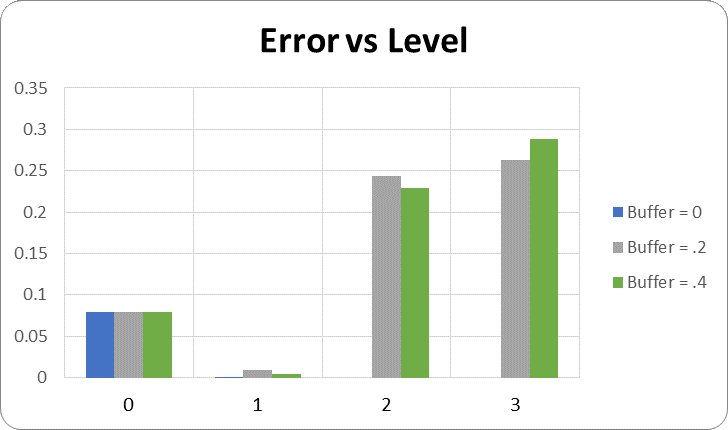
\includegraphics[scale=.5]{convergencechebsinsin.png}
  \caption{Error plateus or increases after level 1}
\end{center}
\end{figure}



Here the $L_1$ error was calculated against the true solution $u = \sin{2\pi y}\frac{\sinh{2 \pi (x-1)} }{\sinh{4\pi}}$

\begin{figure}[H]
\begin{center}
  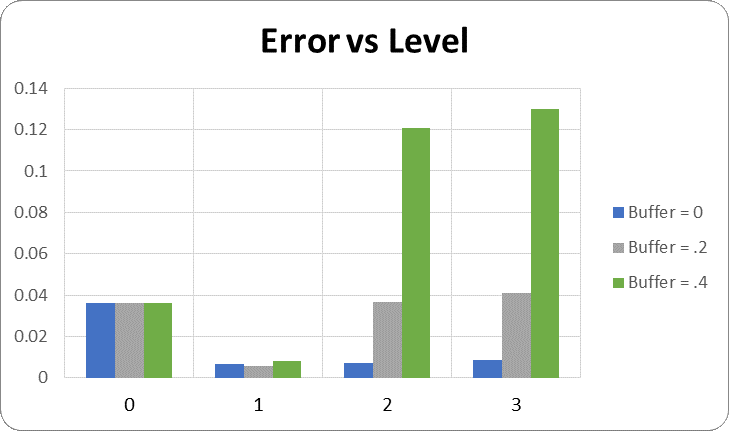
\includegraphics[scale=.5]{convergencechebsinhsin.png}
  \caption{Error plateus or increases after level 1}
\end{center}
\end{figure}


This implementation of SRMG could not consistently achieve error reduction on levels beyond the first level of SRMG, regardless of buffer size, coarse resolution, or number of levels. 

\section{Explanation of Results}
%\section{Concluding Analysis: Iterative SRMG failure}
The underlying assumptions of SRMG require that subsequent levels generate higher-frequency approximations of the true solution. However, low-frequency errors coming from the first level of SRMG seemed to propagate into the interior of all subpatches generated at later levels.  

A new, more careful analysis was done with this problem in mind, leading to a new condition for iterative SRMG.



\subsection{Poisson's Equation on Subdomains}

Consider the uniqueness theorem of Poisson's equation \cite{poissonunique}.

\begin{theorem}
Let $u(\Omega)$ be a solution to Poisson's equation
\begin{align*} 
\nabla^2 u = f\\
\\ u = g \; on \; \partial \Omega 
\end{align*}
$u(\Omega)$ is unique. 
\end{theorem}

 We can also conclude the following corrolary. 

\begin{corollary}
\label{corollaryunique}
On any closed subset of the domain $\tilde{\Omega}_i \subset \Omega$, there is a unique solution v to the following equation. 
\begin{align*} 
\nabla^2 v = f\\
\\ v = u \; on \; \partial \tilde{\Omega}_i 
\end{align*}
$v(\tilde{\Omega}_i)$ is unique. 
Furthermore, $u$, the solution to Poisson's equation on the full domain, restricted to $\tilde{\Omega}_i$ satisfies this equation $\implies v = u$. 
\end{corollary}

% It is therefore possible to solve for $u$ by solving on individual patches, and then constructing a set of indicator functions on $\cup \tilde{\Omega}_i$ such that

% \[ \begin{cases} 
%       1 & x \in \tilde{\Omega}_i \cap  (\cup{\tilde{\Omega}_{j<i}}^c)  \\
%       \\
%       0 & x \in \tilde{\Omega}^c_i \cup{\tilde{\Omega}_{j<i}}
%    \end{cases}
% \]

% \textbf{JRT:Express more clearly how these indicator functions are made. They sort of form a jigsaw. This is a detail I never really revisit, should it just be a remark}
% \subsection{Fourier Projection}

% For simplicity: consider this specific Poisson equation on [0, 1]

% \begin{gather}
%   \bigtriangleup u(x,y) = f  \\
%   \begin{split}
%     u(0,y) &= W(y) \quad u(1,y) =  E(y)\\
%     u(x,0) &= S(x) \quad u(x,1) = N(x) \label{laplaceexboundary}
%   \end{split}
% \end{gather}

% There is a tensor product of orthogonal bases on the domain $[0, 1]x[0,1]$: $S_{i}(x) x S_j(y) = \{\sin{i \pi x}\} \; \times \; \{\sin{j \pi x}\}$  that can satisfy the forcing condition with homogenous boundary conditions.

% There are also corresponding bases that can construct the boundary conditions with homogenous forcing condition.

% \begin{align*}
% % FW_i = \frac{\sinh{i \pi (1-x)}}{\sinh{i \pi }}\sin{i y \pi} \\
% % FE_i = \frac{\sinh{i \pi x}}{\sinh{i \pi }}\sin{i y \pi} \\
% % FS_i = \frac{\sinh{i \pi (1-y) }}{\sinh{i \pi }}\sin{i x \pi} \\
% % FN_i = \frac{\sinh{i \pi y}}{\sinh{i \pi }}\sin{i x \pi} \\
% FW_i = \sinh{i \pi (1-x)}\sin{i y \pi} \\
% FE_i = \sinh{i \pi x} \sin{i y \pi} \\
% FS_i = \sinh{i \pi (1-y)}\sin{i x \pi} \\
% FN_i = \sinh{i \pi y} \sin{i x \pi} \\
% \end{align*}

% Note that there is an ensuing representation of Poisson's equation in the following way


% \begin{gather}
%   \bigtriangleup  \hat{u}[i, j] S_i(x) S_j(y)  = \hat{f}[i, j] S_i(x) S_j(y) \\
%   \begin{split}
%    \hat{u}(0, y)[i]FW_i  &= \hat{W(i)}FW_i  \quad \hat{u}(1,y)[i]FE_i =  \hat{E(i)}FE_i\\
%    \hat{u}(x, 0)[i]FS_i  &= \hat{S(i)}FS_i  \quad \hat{u}(x,1)[i]FN_i =  \hat{N(i)}FN_i\\
%   \end{split}
% \end{gather}

% Therefore our true solution is as follows


% $u = \mathlarger{\sum}_{i,j \in [1, \infty]^2} \hat{u}[i, j] S_i S_j + \mathlarger{\sum}_{i=1}^\infty \hat{u}(0, y)[i] FW_i + \hat{u}(1, y)[i] FE_i + \hat{u}(x, 0)[i] FS_i + \hat{u}(x, 1)[i] FN_i $

% For brevity we again express this as 

% $\sum_{i,j \in [1, \infty]^2} \phi_{i,j}(x, y) + \sum_{i=1}^\infty B_{i}(x, y) = \phi(x, y) + B(x, y)$

% Note this decouples the solution so that the forcing equation and boundary value conditions can be solved for independently. 

% \begin{gather}
%   \bigtriangleup  B(x,y) = 0 \label{laplaceexstate} \\
%   \begin{split}
%     B(0, y) &= W(y) \quad B(1, y) = E(y) \\
%     B(x, 0) &= S(x) \quad B(x, 1) = N(x) \\
%   \end{split}
% \end{gather}

% \begin{gather}
%   \bigtriangleup \phi(x, y) = f  \\
%   \begin{split}
%    \phi(x, y) &= 0 \in  \partial ([0, 1]^2)
%   \end{split}
% \end{gather}




% \subsection{Fourier Approximation}

% Assume that the function $B(x, y)$ can be constructed exactly, but that we can only solve for the first ${N_0} x {N_0}$ bases elements of $\phi_{i,j}$. 

% If these elements are constructed via projection, meaning there is no aliasing error and the coefficient is exact up to the high-frequency terms, then this approximation imposes the following error. 

% \begin{align}
% u^{(0)}(x, y) - u(x, y) &= \phi^{(0)}(x, y) - \phi(x, y) + B(x, y) - B(x, y) \nonumber \\ 
% &=\sum_{i,j=[1, \infty]^2} \hat{u}[i,j] S_i(x) S_j(y) - \sum_{i,j=[1, N_0]^2} \hat{u}[i,j] S_i(x) S_j(y) \nonumber \\
% & = \sum_{i \in [1, \infty]} \sum_{j \in [N_0+1, \infty] } \hat{u}[i, j] S_i(x) S_j(y) \nonumber \\
% & + \sum_{i \in [N_0+1 \infty]} \sum_{j \in [1, \infty]} \hat{u}[i,j] S_i(x) S_j(y) \label{coarseerror}
% \end{align}

\subsection{Recursive SRMG}

Assume the following about the mechanics of SRMG: each subdomain generated by the $l^{th}$ level of SRMG, $\Omega^{l}_i$, is a proper subset of some subdomain $\Omega^{l-1}_j$ with $\Omega^{0} = \Omega$ 

Furthermore assume that on each level of SRMG for $l \geq 1$, a patch solution $u^{(l)}_i$ is approximated to the following Poisson equation:

\begin{gather}
  \bigtriangleup u^{(l)}_i = f \nonumber  \\
  \begin{split}
    u^{(l)}_i = u^{(l-1)}_j \in \partial \Omega^{l}_i \label{patchpdel}
  \end{split}
\end{gather}

Here $u^{(l-1)}_j$ is a solution to a corresponding Poisson equation from a subdomain generated by the previous level of SRMG. That is, each patch is a solution to Poisson's equation with artificial boundary conditions imposed by the solution generated via the previous level of SRMG.



\begin{theorem}
For $l \geq 2$, the analytical solution  $u^{(l)}_i \in  \Omega^{l}_i \subset \Omega^{l-1}_j $ is unique and equals:
$u^{(l-1)}_j \in \Omega^{l-1}_j $.  
\end{theorem}

The above theorem follows directly from \ref{corollaryunique}
 
% \begin{proof}
% Consider $e^{(l)}_i = u^{(l)}_i - u^{(l-1)}_j$
% \begin{gather*}
%   \bigtriangleup e^{(l)}_i = \bigtriangleup u^{(l)}_i - \bigtriangleup u^{l-1}_j = f-f = 0   \\
%   \begin{split}
%    e^{(l)}_i =  u^{(l)}_i - u^{(l-1)}_j = 0 \in \partial (\Omega^{(l)}_i)
%   \end{split}
% \end{gather*}

% Thus $e^{(l)}$ is the solution to the homogenous Poisson equation, which means $0 = e^{(l)}  \implies u^{(l)}_i - u^{(l-1)}  = 0 \implies u^{(l)}_i = u^{(l-1)}_j$

% \end{proof}

\begin{corollary}
The analytical solution to the equations governing any $u^{(l)}_i$ is given by the solution $u^{(1)}_j$ where $\Omega^{l}_i \subset \Omega^{1}_j$
\end{corollary}

The direct result of this is that $e^{(l)}_i = u^{(l)}_i - u = u^{(1)}_j - u = e^{(1)}_j$. That is, the pointwise error induced by imposing artificial boundary conditions on level 1 has an effect on all subsequent levels of Segmental Refinement. 

This contradicts one of our fundamental requirements of SRMG, that high-frequency errors on the interior of a patch could be eliminated by refinement. Unfortunately, error imposed by the first artificial boundary cannot be eliminated by anything other than a more refined coarse solve, or a suitably large buffer. The required size of this buffer grows to accommodate the stronger convergence requirements on higher-resolution grids. 

%So guaranteeing second-order discretization error still allows low-magnitude and low-frequency error on the interior of subpatches, meaning the buffer size required by SRMG to induce second-order discretization error with respect to a given refinement grows proportional to total refinement desired. 

%Therefore the pointwise error induced on any subpatch can only be reduced by reducing error on the first level of SRMG in the patch $\Omega^{(1)}_i$ that contains the subpatch corresponding to $\Omega^{(l)}_j$. %Reducing the error on the first level of SRMG can only be done by increasing the first-level buffer region or the coarse resolution.

%However, note that we have the same guarantees about the decay of error as described in previous sections. Although the pointwise error on a subdomain can't be reduced by refinement or choice of solver, we can still get stronger convergence guarantees on later patches by assuring a buffer that grows. 


\subsection{Error Analysis Revisited}

Note that our original analysis holds the for the first level of Segmental Refinement. If $u^{(0)} - u$ contains primarily high frequncies, then the first artificial boundaries induced by SRMG impose second-order discretization error with a suitably large buffer. The problem is that further levels of SRMG still encode this error, and this error decays no faster on later levels, regardless of refinement. 

Therefore, SRMG requires not just that $e^{(0)} \leq \frac{C_D}{N_0^2}$, but that $e^{(0)} \leq \epsilon $, where $\epsilon$ is the target accuracy at the finest level of SRMG. 

We revisit just the first-level buffer requirements, given by (\ref{bufferreq}), but with the updated requirement on $d_1$ that $e^{(0)} \leq \epsilon $ 

\begin{align*}
d_1 &> \frac{ 5\ln{2} + \ln{C} + \ln{N_0} - \ln{ \epsilon}  }{2 N_0 \pi } \\
%d_1 &> \frac{\ln(C) - \ln{(4^{-S} C_D \cdot S) } +(4+3)\ln2 + 3\ln{N_0} }{2 N_0 \pi}\\
%  & = \frac{\ln(C)- \ln{C_D } + 3\ln{N_0}+ (7+2S)\ln2 + \ln{S} }{2 N_0 \pi} 
\end{align*}


%We again study $\overline{d_l} = \sum_{i=l}^\infty d_i$, the total buffer required at each level to perform further refinements.


\begin{align*}
\overline{d_l} &= \sum_{i=l}^\infty d_i \\ 
%& = \frac{ln2}{2 N_0 \pi } 2^{1-l}(l+5) + \frac{\ln{C} + \ln{N_0} -\ln{\epsilon_{mach}} }{2 N_0 \pi}\\
%& = \frac{2\ln{2}* 2^{-l}(l+5) + \ln{C} + \ln{N_0} - \ln{\epsilon_{mach} }  }{2 N_0 \pi }
& = \frac{ln2}{2 N_0 \pi } 2^{1-l}(l+5) + 2^{1-l}\frac{\ln{C} + \ln{N_0} -\ln{\epsilon}}{ N_0 \pi}\\
& = \frac{2^{1-l}}{N_0 \pi } \left( \frac{(l+5)\ln2 }{2} + \ln C + \ln{N_0} - \ln{\epsilon} \right)
%\frac{\ln{2}(4+l) + \ln{C} + \ln{N_0} -\ln{\epsilon_{mach}} }{N_0 \pi 2^l} 
\end{align*}


An extremely important thing to note is that this analysis crucially relies on no low-frequency error being introduced by any subsequent level of SRMG. This may cause failure to converge not only on this given patch, but on any subsequent subdomain, since my analsis has shown that no method of refinement will eliminate this error. 

Therefore, we still must consider an implementation that remedies all sources of low-frequency error including aliasing error, interpolation error, or limitations of the basis used to represent each patch solution.


\subsection{Conclusion}\label{sec:conc}

Previous analysis and work relied on the assumption that if each level of SRMG could guarantee error on the same order of magnitude as traditional multigrid, then it would also inherit the multigrid property that this error would be restricted to higher frequencies. This property on the frequency of error does not hold in SRMG. Even if we make the extremely optimistic assumption that we can generate the exact solution to each patch's PDE, it is clear that the error induced by the first iteration of Segmental Refinement induces error that cannot be restricted to higher frequencies. Thus, the first buffer region must grow to accomodate the final desired error. 

Computational resources and/or a suitably optimized spectral solver were not available to test the newfound convergence requirements. However, we have shown here several numerical experiments and a rigorous analysis of Segmental Refinement. All are consistent with previous work, where the buffer size had to grow to accommodate further levels of SRMG. I have also shown potential solutions for this issue, although the feasibility of these solutions is yet to be determined. 

Iterative Segmental Refinement only guarantees convergence if there is no reintroduction of low-frequency error via interpolation, no low-frequency error due to aliasing, and a buffer size large enough to eliminate error induced by the first (and each subsequent) artificial boundary.  

These are requirements that are much more difficult to satisfy than those posed by our original justification. However, in the case that these requirements are not feasible, Segmental Refinement is still suitable for a few of the finest levels assuming a large buffer is chosen. My analysis here demonstrates possible points of failure and methods to ameloriate them. 



\bibliographystyle{siamplain}
\bibliography{references}

\end{document}
